\documentclass{standalone}

\usepackage[dvipsnames]{xcolor}
\usepackage{tikz}

\usetikzlibrary{calc} % to compute rectangle coords on the fly
\usetikzlibrary{positioning} % for below of=
\usepackage{kpfonts}


\begin{document}

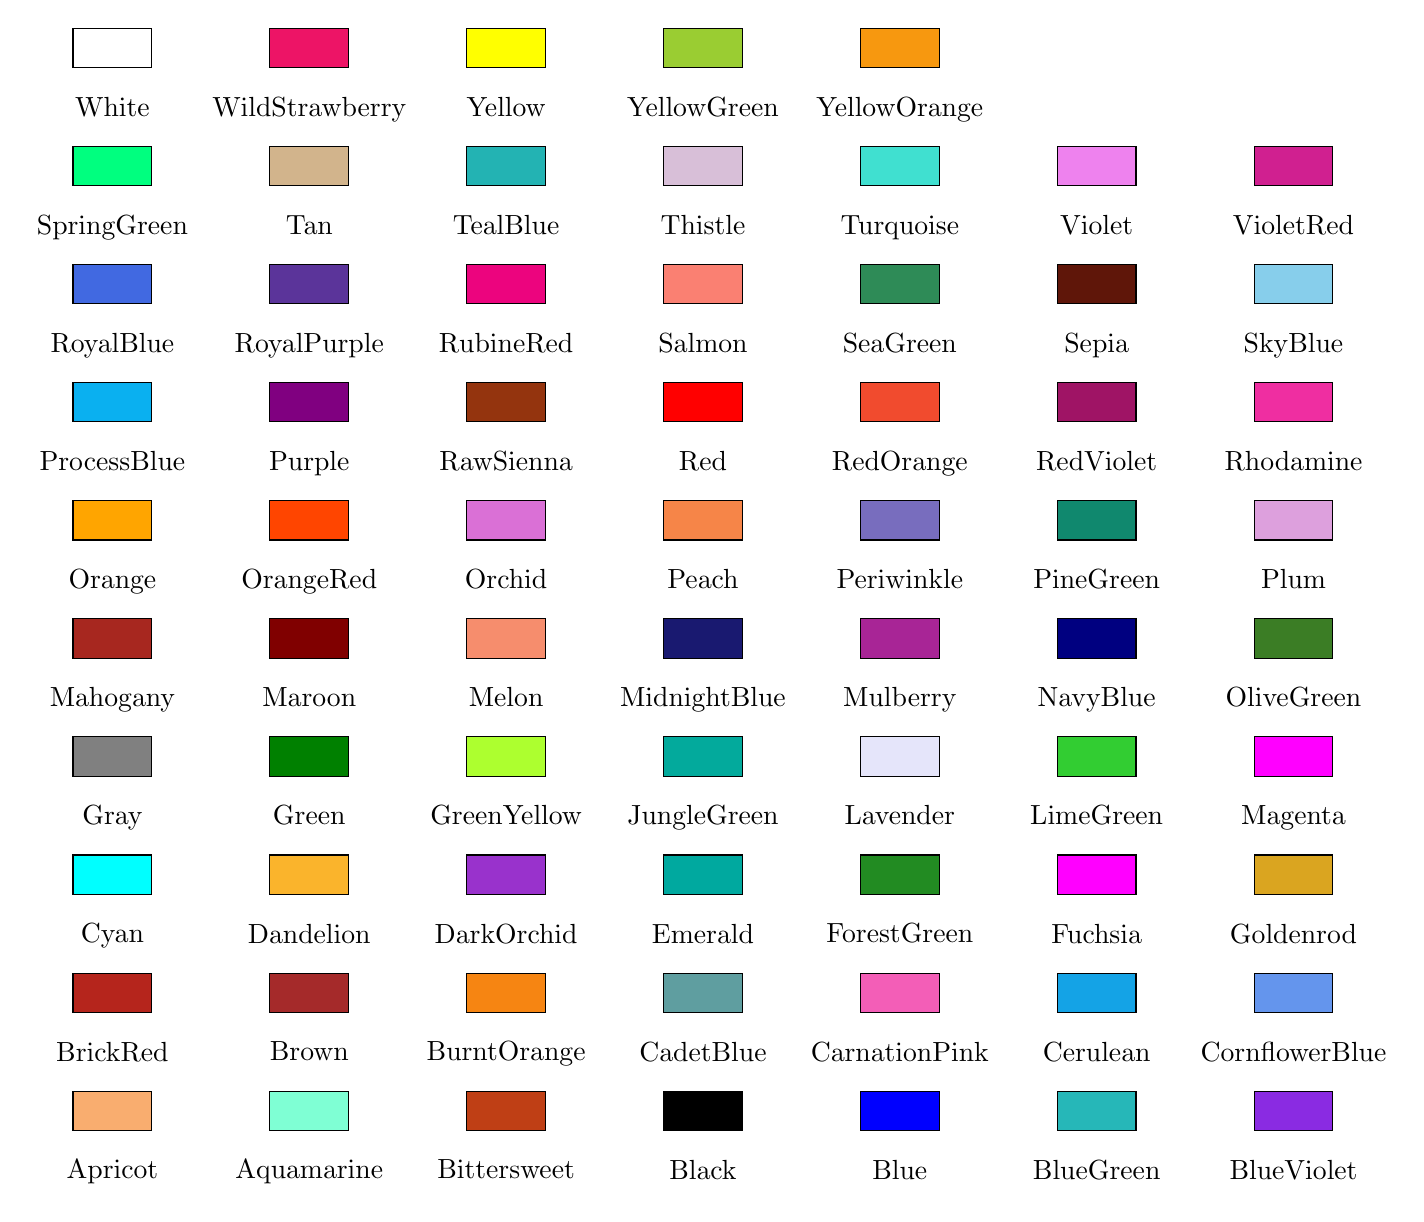
\begin{tikzpicture}
    \def \columnWidth {7};
    \def \baseWidth {0.5cm};
    \def \baseHeight {0.25cm};

    \foreach \color [count=\i from 0] in {
        Apricot, Aquamarine, Bittersweet, Black, Blue, BlueGreen, BlueViolet, BrickRed,
        Brown, BurntOrange, CadetBlue, CarnationPink, Cerulean, CornflowerBlue, Cyan,
        Dandelion, DarkOrchid, Emerald, ForestGreen, Fuchsia, Goldenrod, Gray, Green,
        GreenYellow, JungleGreen, Lavender, LimeGreen, Magenta, Mahogany, Maroon, Melon,
        MidnightBlue, Mulberry, NavyBlue, OliveGreen, Orange, OrangeRed, Orchid, Peach,
        Periwinkle, PineGreen, Plum, ProcessBlue, Purple, RawSienna, Red, RedOrange,
        RedViolet, Rhodamine, RoyalBlue, RoyalPurple, RubineRed, Salmon, SeaGreen,
        Sepia, SkyBlue, SpringGreen, Tan, TealBlue, Thistle, Turquoise, Violet,
        VioletRed, White, WildStrawberry, Yellow, YellowGreen, YellowOrange} {

        \coordinate (center_\color)
                        at ({2.5*mod(\i, \columnWidth)}, {1.5*div(\i, \columnWidth)});
        \coordinate (rectangle_bottom_\color)
                        at ($(center_\color) - (\baseWidth, \baseHeight)$);
        \coordinate (rectangle_top_\color)
                        at ($(center_\color) + (\baseWidth, \baseHeight)$);
        
        \draw[fill=\color, black] (rectangle_bottom_\color) rectangle (rectangle_top_\color);
        \node[below=0.5cm of center_\color] {\color};
    }
\end{tikzpicture}

\end{document}
